% chapter02.tex

 %%%%%%%%%%%%%%%%%%%%%%%%%%%%%%%%%%%%%%%%%%%%%%%%%%%%%%%%%%%%%%%%%%%%%%%%%%%%%
 %                                                                           %
 %    PyMS documentation                                                     %
 %    Copyright (C) 2005-8 Vladimir Likic                                    %
 %                                                                           %
 %    The files in this directory provided under the Creative Commons        %
 %    Attribution-NonCommercial-NoDerivs 2.1 Australia license               %
 %    http://creativecommons.org/licenses/by-nc-nd/2.1/au/                   %
 %    See the file license.txt                                               %
 %                                                                           %
 %%%%%%%%%%%%%%%%%%%%%%%%%%%%%%%%%%%%%%%%%%%%%%%%%%%%%%%%%%%%%%%%%%%%%%%%%%%%%

\chapter{Using PyMS}

\section{Introduction}

This chapter gives examples of PyMS use. The commands used in the examples
are collected into scripts and saved in the project 'pyms-test'.  Each example
subsection given below has a corresponding directory in 'pyms-test'. The
project 'pyms-data' contains data files used in all examples. Both 'pyms-data'
and 'pyms-test' are downloadable from Google Code.

The setup used for the examples below is as follows. The projects 'pyms',
'pyms-data', and 'pyms-test' were all downloaded in the directory
{\tt /home/current/proj/PyMS}. In each example the Python interpreter
was made aware of the PyMS location with the following commands:

\begin{verbatim}
>>> import sys
>>> sys.path.append("/home/current/proj/PyMS/")
\end{verbatim}

For brevity these commands will not be shown in the examples below.

Each example was run from the corresponding sub-directory of 'pyms-test':
Example 1 was run in {\tt pyms-test/example01}, and so on.

\section{PyMS examples}

\subsection{Example 1: Reading GC-MS data exported from Agilent ChemStation}

The PyMS package pyms.IO provides capabilities to read the raw GC-MS
data stored in the ANDI-MS format. The function IO.ANDI.ChemStation()
provides the interface to ANDI-MS data files saved from Agilent
ChemStation software. The name is a reminder that this function has
been tested only on the data exported from Agilent ChemStation.

ANDI-MS data format stands for Analytical Data Interchange for Mass
Spectrometry, and was developed for the description of mass spectrometric
data developed in 1994 by Analytical Instrument Association. ANDI-MS 
is essentially a recommendation, and it is up to individual vendors of
mass spectrometry processing software to implement "export to ANDI-MS"
feature in their software. Furthermore, it is vendor's good will to
implement ANDI-MS specifications properly. Because of these limitations
one cannot be certain that one can properly read ANDI-MS files from
a particular vendor without testing this first.

The file '0510\_217.CDF' is a GC-MS experiment exported from Agilent
ChemStation (located in 'pyms-data'). This file can be loaded in the
memory as follows:

\begin{verbatim}
>>> from pyms.IO.ANDI.Class import ChemStation
>>> andi_file = "/home/current/proj/PyMS/pyms-data/0510_217.CDF"
>>> data = ChemStation(andi_file)
 -> Processing netCDF file '/home/current/proj/PyMS/pyms-data/0510_217.CDF'
    [ 2784 scans, masses from 50 to 550 ]
>>>
\end{verbatim}

\noindent
The above command creates the object 'data' which is an {\em instance}
of the class IO.ANDI.ChemStation.  The instance 'data' has several
attributes and methods associated with it.

\subsection{Example 2: Exploring data attributes}

Load the data as shown in the Example 2.

The method {\tt get\_filename()} returns the name of the file from which
the data was loaded. Usage example:

\begin{verbatim}
>>> print data.get_filename()
/home/current/proj/PyMS/pyms-data/0510_217.CDF
\end{verbatim}

The method {\tt get\_ic\_at\_index(i)} returns an IonChromatogram object
at index i. For example, to get the first ion chromatogram from the data
matrix:

\begin{verbatim}
>>> ic = data.get_ic_at_index(1)
\end{verbatim}

\noindent
An IonChromatogram object is the one dimensional time vector containing
mass intensities as a function of retention time.

An ion chromatogram is a set of intensities as a function of retention
time. This can can be either m/z channel intensities (for example, ion
chromatograms at m/z = 65), or cumulative intensities over all measured
m/z. In the latter case the ion chromatogram is total ion chromatogram
(TIC).

The nature of an IonChromatogram object can be revealed by calling
the method .is\_tic():

\begin{verbatim}
>>> print ic.is_tic()
False
\end{verbatim}

\noindent
This shows that the first ion chromatogram in the data file is for
m/z = 51.

\begin{verbatim}
>>> tic = data.get_tic()
>>> print tic.is_tic()
True
\end{verbatim}

\noindent
This shows the method to obtain a TIC from the data. Note that both
'ic' and 'tic' are instances of the IonChromatogram class.

The method {\tt get\_ic\_at\_mass(mz)} returns an IonChromatogram
object corresponding to given m/z. For example, to get the ion
chromatogram that corresponds to m/z = 73:

\begin{verbatim}
>>> ic = data.get_ic_at_mass(73)
>>> print ic.is_tic()
False
\end{verbatim}

The method {\tt get\_intensity\_matrix()} returns the entire matrix of
intensities:

\begin{verbatim}
>>> im = data.get_intensity_matrix()
>>> print len(im)
2784
>>> print len(im[0])
501
\end{verbatim}

\noindent
This data matrix contains 2784 time points (MS scans), and each time point
corresponds to a mass spectrum of 501 m/z points.

\subsection{Example 3: How to write data to external files}

Load the data as shown in the Example 2.

Get the TIC as shown in Example 2 and save to a file:

\begin{verbatim}
>>> ic = data.get_tic()
>>> ic.write("output/tic.dat")
\end{verbatim}

\noindent
The TIC will be written as a number of pairs (retention time, intensity),
with one such pair per line:

\begin{verbatim}
$ cat tic.dat
 305.666      745997
 306.009      726566
 306.352      717704
 306.695      684214
 307.038      701866
 307.381      893306
 307.724     1278099
 308.067     1290984
 308.410      925558
 308.752      644122
[..output deleted..]
\end{verbatim}

\noindent
The left column is the retention time in seconds, while the right column
is the corresponding intensity. This data can be conveniently loaded and
plotted in matlab or octave:

\begin{verbatim}
octave:1> load tic.dat
octave:2> plot(tic(:,1)/60, tic(:,2))
\end{verbatim}

The output is shown in Figure \ref{ticplot}. In the above command the
time was divided by 60 to convert the x-axis into minutes.

\begin{figure}[htp]
\begin{center}
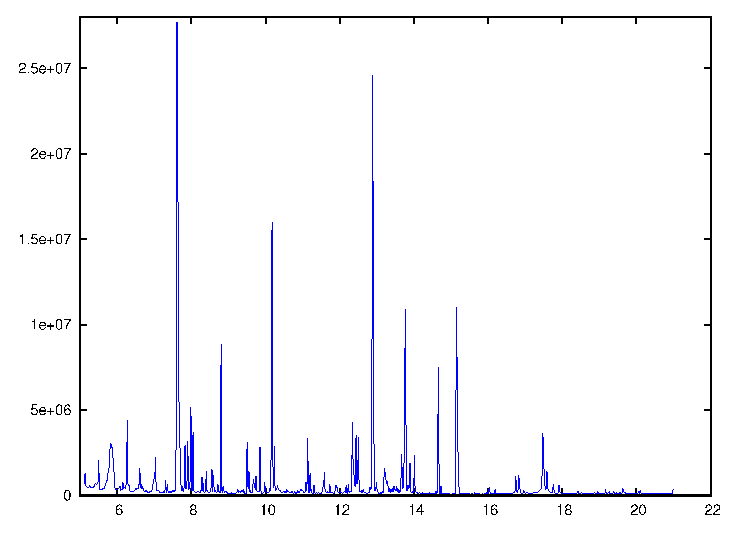
\includegraphics{graphics/tic.eps}
\caption{The octave plot of the file 'tic.dat'.}
\label{ticplot}
\end{center}
\end{figure}

To get the intensity matrix and save to a file:

\begin{verbatim}
>>> im = data.get_intensity_matrix()
>>> save_data("output/im.dat", im)
\end{verbatim}

\noindent
The TIC can of course be calculated from the intensity matrix. For a quick
check whether the intensity matrix matches the TIC one can use matlab or
octave:

\begin{verbatim}
octave:1> load tic.dat
octave:2> load im.dat
octave:3> v1 = tic(:,2)';
octave:4> v2 = sum(im');
octave:6> sum(abs(v1-v2))
ans = 0
\end{verbatim}

Alternatively, one can export the entire data into the CSV format by
calling the methods export\_csv():

\begin{verbatim}
>>> data.export_csv("output/data")
\end{verbatim}

\noindent
This will create the files 'data.im.csv', 'data.mz.csv', and 'data.rt.csv'
in the directory output/, where these are the intensity matrix, retention
time vector, and m/z vector in the CSV format, respectively.

